% =============================================================================
% Module 7.0: Network Services and High Availability
% Network+ Course - LaTeX Beamer Presentation
% Theme: It's Always Sunny in Philadelphia
% =============================================================================

\documentclass[aspectratio=169, 11pt]{beamer}

% Theme and colors
\usetheme{Madrid}
\usecolortheme{default}

% Custom colors - RCTC and Network theme
\definecolor{rctcblue}{RGB}{0, 74, 136}
\definecolor{rctcgold}{RGB}{255, 199, 44}
\definecolor{networkgreen}{RGB}{0, 150, 100}
\definecolor{alertred}{RGB}{200, 50, 50}
\definecolor{aborange}{RGB}{230, 120, 0}
\definecolor{tcpblue}{RGB}{30, 100, 180}
\definecolor{udpgreen}{RGB}{50, 160, 80}
\definecolor{dhcppurple}{RGB}{120, 60, 160}
\definecolor{dnsyellow}{RGB}{200, 170, 50}
\definecolor{paddysgreen}{RGB}{0, 100, 60}
\definecolor{phillyblue}{RGB}{0, 43, 92}
\definecolor{sunnyorange}{RGB}{255, 140, 0}

% Set theme colors
\setbeamercolor{palette primary}{bg=rctcblue, fg=white}
\setbeamercolor{palette secondary}{bg=rctcblue!80, fg=white}
\setbeamercolor{palette tertiary}{bg=rctcblue!60, fg=white}
\setbeamercolor{structure}{fg=rctcblue}
\setbeamercolor{title}{fg=white, bg=rctcblue}
\setbeamercolor{frametitle}{fg=rctcblue, bg=rctcblue!10}
\setbeamercolor{block title}{bg=rctcblue, fg=white}
\setbeamercolor{block body}{bg=rctcblue!5}
\setbeamercolor{block title alerted}{bg=alertred, fg=white}
\setbeamercolor{block body alerted}{bg=alertred!5}
\setbeamercolor{block title example}{bg=networkgreen, fg=white}
\setbeamercolor{block body example}{bg=networkgreen!5}

% Packages
\usepackage{tikz}
\usepackage{booktabs}
\usepackage{fontawesome5}
\usepackage{graphicx}
\usepackage{xcolor}
\usepackage{colortbl}
\usepackage{array}
\usepackage{listings}
\usepackage{amsmath}
\usepackage{amssymb}

% TikZ libraries
\usetikzlibrary{shapes.geometric, arrows.meta, positioning, decorations.pathreplacing, 
                backgrounds, fit, calc, shadows, shapes.symbols, shapes.misc}

% Custom TikZ styles for network diagrams
\tikzstyle{pc} = [inner sep=0pt]
\tikzstyle{laptop} = [inner sep=0pt]
\tikzstyle{server} = [inner sep=0pt]
\tikzstyle{router} = [inner sep=0pt]
\tikzstyle{switch} = [inner sep=0pt]
\tikzstyle{firewall} = [inner sep=0pt]
\tikzstyle{cloud} = [inner sep=0pt]
\tikzstyle{phone} = [inner sep=0pt]

% Connection styles
\tikzstyle{ethernet} = [draw, line width=1.5pt, color=rctcblue, -{Stealth}]
\tikzstyle{ethernet noarrow} = [draw, line width=1.5pt, color=rctcblue]
\tikzstyle{wireless} = [draw, line width=1.5pt, color=networkgreen, dashed, -{Stealth}]
\tikzstyle{wan} = [draw, line width=2pt, color=aborange, -{Stealth}]
\tikzstyle{wan noarrow} = [draw, line width=2pt, color=aborange]
\tikzstyle{secure} = [draw, line width=1.5pt, color=paddysgreen, -{Stealth}]

% Packet/segment styles
\tikzstyle{pktseg} = [draw=rctcblue, fill=rctcblue!10, minimum height=0.5cm, 
                      font=\tiny, rounded corners=2pt]
\tikzstyle{pktseg tcp} = [draw=tcpblue, fill=tcpblue!15, minimum height=0.5cm, 
                          font=\tiny, rounded corners=2pt]
\tikzstyle{pktseg udp} = [draw=udpgreen, fill=udpgreen!15, minimum height=0.5cm, 
                          font=\tiny, rounded corners=2pt]
\tikzstyle{pktseg highlight} = [draw=aborange, fill=aborange!20, minimum height=0.5cm, 
                                font=\tiny, rounded corners=2pt]

% Box styles
\tikzstyle{ipbox} = [draw=rctcblue, fill=rctcblue!10, rounded corners, 
                     minimum height=0.4cm, font=\small]
\tikzstyle{portbox} = [draw=tcpblue, fill=tcpblue!10, rounded corners,
                       minimum height=0.4cm, font=\small]
\tikzstyle{tlsbox} = [draw=paddysgreen, fill=paddysgreen!15, rounded corners,
                      minimum height=0.4cm, font=\small]

% Process/flow styles
\tikzstyle{process} = [draw=rctcblue, fill=rctcblue!15, rounded corners,
                       minimum width=2cm, minimum height=0.6cm, font=\small, align=center]
\tikzstyle{decision} = [draw=aborange, fill=aborange!15, diamond, aspect=2,
                        minimum width=1.5cm, font=\small, align=center]

% Icon commands using FontAwesome
\newcommand{\iconpc}[1][0.6cm]{\resizebox{#1}{!}{\faDesktop}}
\newcommand{\iconlaptop}[1][0.6cm]{\resizebox{#1}{!}{\faLaptop}}
\newcommand{\iconserver}[1][0.6cm]{\resizebox{#1}{!}{\faServer}}
\newcommand{\iconrouter}[1][0.6cm]{\resizebox{#1}{!}{\faNetworkWired}}
\newcommand{\iconswitch}[1][0.6cm]{\resizebox{#1}{!}{\faSitemap}}
\newcommand{\iconfirewall}[1][0.6cm]{\resizebox{#1}{!}{\faIcon{shield-alt}}}
\newcommand{\iconcloud}[1][0.6cm]{\resizebox{#1}{!}{\faCloud}}
\newcommand{\iconphone}[1][0.6cm]{\resizebox{#1}{!}{\faPhone}}
\newcommand{\icondatabase}[1][0.6cm]{\resizebox{#1}{!}{\faDatabase}}
\newcommand{\iconglobe}[1][0.6cm]{\resizebox{#1}{!}{\faGlobe}}
\newcommand{\iconuser}[1][0.6cm]{\resizebox{#1}{!}{\faUser}}
\newcommand{\iconlock}[1][0.6cm]{\resizebox{#1}{!}{\faLock}}
\newcommand{\iconclock}[1][0.6cm]{\resizebox{#1}{!}{\faClock}}
\newcommand{\iconmail}[1][0.6cm]{\resizebox{#1}{!}{\faEnvelope}}
\newcommand{\iconvoip}[1][0.6cm]{\resizebox{#1}{!}{\faPhoneVolume}}

% Key term formatting
\newcommand{\keyterm}[1]{\textbf{\textcolor{rctcblue}{#1}}}

% Case study environments - Sunny theme
\newenvironment{casestudy}[1]{%
    \begin{alertblock}{#1}
}{\end{alertblock}}

\newenvironment{casesolution}[1]{%
    \begin{exampleblock}{Solution: #1}
}{\end{exampleblock}}

% Document info
\title[Module 7.0]{Module 7.0: Network Services and High Availability}
\subtitle{Network+ Certification Course}
\author{Brendan Shea, PhD}
\date{Introduction to Networking}
\institute{RCTC}

\begin{document}

% =============================================================================
% SLIDE 1: Title Slide
% =============================================================================
\begin{frame}
    \titlepage
    \begin{center}
        \begin{tikzpicture}[scale=0.6]
            % Client
            \node[pc] (client) at (0,0) {\iconpc[0.5cm]};
            \node[font=\tiny, below=0.05cm of client] {Client};
            
            % TLS Lock
            \node (lock) at (2.5,0.5) {\iconlock[0.4cm]};
            \node[font=\tiny, paddysgreen, below=0.02cm of lock] {TLS};
            
            % Web Server
            \node[server] (web) at (5,0) {\iconserver[0.4cm]};
            \node[font=\tiny, above=0.02cm of web] {Web};
            
            % Database
            \node (db) at (7.5,0) {\icondatabase[0.4cm]};
            \node[font=\tiny, below=0.05cm of db] {Database};
            
            % HA Servers
            \node[server] (ha1) at (10,0.5) {\iconserver[0.35cm]};
            \node[server] (ha2) at (10,-0.5) {\iconserver[0.35cm]};
            \node[font=\tiny, right=0.1cm of ha1] {HA};
            
            % Connections
            \draw[secure] (client) -- (lock);
            \draw[secure] (lock) -- (web);
            \draw[-{Stealth}, tcpblue, line width=1pt] (web) -- (db);
            \draw[-{Stealth}, aborange, line width=1pt] (db) -- (ha1);
            \draw[-{Stealth}, aborange, line width=1pt] (db) -- (ha2);
            
            % Clock for NTP
            \node at (2.5, -1) {\iconclock[0.3cm]};
            \node[font=\tiny] at (2.5, -1.4) {NTP};
        \end{tikzpicture}
    \end{center}
\end{frame}

% =============================================================================
% SLIDE 2: Review - Building on Module 6
% =============================================================================
\begin{frame}{Review: Building on Module 6}
    \begin{columns}[T]
        \begin{column}{0.48\textwidth}
            \begin{block}{What We Learned (Module 6)}
                \small
                \begin{itemize}\setlength{\itemsep}{2pt}
                    \item \textbf{TCP/UDP}: Transport protocols and ports
                    \item \textbf{DHCP}: DORA process for IP assignment
                    \item \textbf{DNS}: Name resolution and record types
                    \item \textbf{Ports}: Service identification (0--65535)
                \end{itemize}
            \end{block}
            
            \vspace{0.3em}
            \begin{alertblock}{The Next Questions}
                \small
                How do we \textbf{secure} these services? How do we keep them \textbf{available}? How do we \textbf{synchronize time} across the network?
            \end{alertblock}
        \end{column}
        \begin{column}{0.48\textwidth}
            \begin{center}
                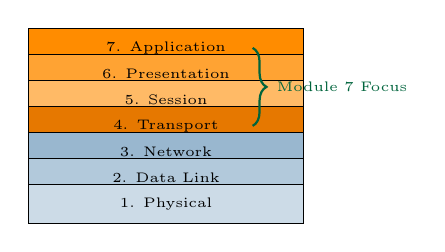
\begin{tikzpicture}[scale=0.55]
                    % OSI layers - highlight 4-7
                    \foreach \i/\name/\color in {
                        7/Application/sunnyorange,
                        6/Presentation/sunnyorange!80,
                        5/Session/sunnyorange!60,
                        4/Transport/aborange,
                        3/Network/rctcblue!40,
                        2/Data Link/rctcblue!30,
                        1/Physical/rctcblue!20
                    } {
                        \node[draw, fill=\color, minimum width=3.5cm, minimum height=0.5cm, 
                              font=\tiny] at (0, \i*0.6-0.6) {\i. \name};
                    }
                    \draw[decorate, decoration={brace, amplitude=5pt, mirror}, thick, paddysgreen]
                        (2, 1.8) -- (2, 3.6) node[midway, right=5pt, font=\tiny, paddysgreen] {Module 7 Focus};
                \end{tikzpicture}
            \end{center}
            
            \vspace{0.2em}
            \begin{exampleblock}{Module 7 Topics}
                \small
                TLS, NTP, HTTP(S), FTP, SMB, Email, VoIP, Disaster Recovery, High Availability
            \end{exampleblock}
        \end{column}
    \end{columns}
\end{frame}

% =============================================================================
% SLIDE 3: Module 7 Learning Objectives
% =============================================================================
\begin{frame}{Module 7 Learning Objectives}
    \begin{columns}[T]
        \begin{column}{0.48\textwidth}
            \begin{block}{1. Security \& Time Sync}
                \small
                \begin{itemize}\setlength{\itemsep}{1pt}
                    \item Transport Layer Security (TLS)
                    \item Network Time Protocol (NTP)
                    \item Precision Time Protocol (PTP)
                \end{itemize}
                \centering\iconlock[0.5cm]\quad\iconclock[0.5cm]
            \end{block}
            
            \vspace{0.2em}
            \begin{block}{2. Web, File \& Database}
                \small
                \begin{itemize}\setlength{\itemsep}{1pt}
                    \item HTTP/HTTPS and web services
                    \item FTP, SFTP, SMB file transfer
                    \item NAS and database connectivity
                \end{itemize}
                \centering\iconglobe[0.5cm]\quad\iconserver[0.5cm]
            \end{block}
        \end{column}
        \begin{column}{0.48\textwidth}
            \begin{block}{3. Email \& Voice Services}
                \small
                \begin{itemize}\setlength{\itemsep}{1pt}
                    \item SMTP, IMAP, POP3
                    \item VoIP protocols (SIP, RTP)
                    \item QoS for voice traffic
                \end{itemize}
                \centering\iconmail[0.5cm]\quad\iconvoip[0.5cm]
            \end{block}
            
            \vspace{0.2em}
            \begin{block}{4. DR \& High Availability}
                \small
                \begin{itemize}\setlength{\itemsep}{1pt}
                    \item RTO, RPO, and DR sites
                    \item Load balancing and clustering
                    \item First Hop Redundancy (FHRP)
                \end{itemize}
                \centering\iconfirewall[0.5cm]\quad\iconrouter[0.5cm]
            \end{block}
        \end{column}
    \end{columns}
\end{frame}

% =============================================================================
% SLIDE 4: Section 7.1 Overview - Security & Time
% =============================================================================
\begin{frame}{Section 7.1: Application Security and Time Synchronization}
    \begin{columns}[T]
        \begin{column}{0.48\textwidth}
            \begin{block}{Why Application Security?}
                \small
                \begin{itemize}\setlength{\itemsep}{2pt}
                    \item Data in transit must be encrypted
                    \item Authentication verifies identity
                    \item Integrity ensures data isn't modified
                    \item TLS provides all three!
                \end{itemize}
            \end{block}
            
            \vspace{0.2em}
            \begin{block}{Why Time Matters}
                \small
                \begin{itemize}\setlength{\itemsep}{2pt}
                    \item Certificate validation requires accurate time
                    \item Log correlation across systems
                    \item Kerberos authentication (5-min tolerance!)
                    \item Scheduled tasks and backups
                \end{itemize}
            \end{block}
        \end{column}
        \begin{column}{0.48\textwidth}
            \begin{center}
                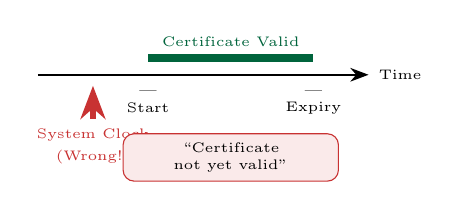
\begin{tikzpicture}[scale=0.7]
                    % Timeline showing cert failure
                    \draw[-{Stealth}, thick] (0,0) -- (6,0) node[right, font=\tiny] {Time};
                    
                    % Cert valid period
                    \draw[paddysgreen, line width=3pt] (2,0.3) -- (5,0.3);
                    \node[font=\tiny, paddysgreen] at (3.5, 0.6) {Certificate Valid};
                    
                    % System clock (wrong)
                    \draw[alertred, -{Stealth}, line width=2pt] (1, -0.8) -- (1, -0.2);
                    \node[font=\tiny, alertred] at (1, -1.1) {System Clock};
                    \node[font=\tiny, alertred] at (1, -1.5) {(Wrong!)};
                    
                    % Markers
                    \node[font=\tiny] at (2, -0.3) {|};
                    \node[font=\tiny] at (2, -0.6) {Start};
                    \node[font=\tiny] at (5, -0.3) {|};
                    \node[font=\tiny] at (5, -0.6) {Expiry};
                    
                    % Error message
                    \node[draw=alertred, fill=alertred!10, rounded corners, font=\tiny, 
                          text width=2.5cm, align=center] at (3.5, -1.5) 
                          {``Certificate not yet valid''};
                \end{tikzpicture}
            \end{center}
            
            \vspace{0.3em}
            \begin{alertblock}{Key Insight}
                \small
                If your clock is wrong, \textbf{nothing works}---certificates fail, logs are useless, and authentication breaks!
            \end{alertblock}
        \end{column}
    \end{columns}
\end{frame}

% =============================================================================
% SLIDE 5: Transport Layer Security (TLS) - Overview
% =============================================================================
\begin{frame}{Transport Layer Security (TLS) --- Overview}
    \begin{columns}[T]
        \begin{column}{0.48\textwidth}
            \begin{block}{What is TLS?}
                \small
                \keyterm{TLS} (Transport Layer Security) is a cryptographic protocol that provides:
                \begin{itemize}\setlength{\itemsep}{1pt}
                    \item \textbf{Encryption}: Data privacy
                    \item \textbf{Authentication}: Server (and optionally client) identity
                    \item \textbf{Integrity}: Data hasn't been tampered with
                \end{itemize}
            \end{block}
            
            \vspace{0.2em}
            \begin{block}{TLS Versions}
                \small
                \begin{itemize}\setlength{\itemsep}{1pt}
                    \item SSL 2.0/3.0 --- \textcolor{alertred}{Deprecated, insecure}
                    \item TLS 1.0/1.1 --- \textcolor{alertred}{Deprecated 2020}
                    \item TLS 1.2 --- Still widely used
                    \item TLS 1.3 --- Current standard (2018)
                \end{itemize}
            \end{block}
        \end{column}
        \begin{column}{0.48\textwidth}
            \begin{center}
                \begin{tikzpicture}[scale=0.65]
                    % Client
                    \node[pc] (client) at (0, 3) {\iconpc[0.5cm]};
                    \node[font=\tiny] at (0, 2.5) {Client};
                    
                    % Server
                    \node[server] (server) at (4, 3) {\iconserver[0.5cm]};
                    \node[font=\tiny] at (4, 2.5) {Server};
                    
                    % Handshake steps
                    \draw[-{Stealth}, tcpblue, line width=1pt] (0.3, 2.3) -- (3.7, 2) 
                        node[midway, above, font=\tiny, sloped] {1. Client Hello};
                    \draw[-{Stealth}, paddysgreen, line width=1pt] (3.7, 1.6) -- (0.3, 1.3) 
                        node[midway, above, font=\tiny, sloped] {2. Server Hello + Cert};
                    \draw[-{Stealth}, aborange, line width=1pt] (0.3, 0.9) -- (3.7, 0.6) 
                        node[midway, above, font=\tiny, sloped] {3. Key Exchange};
                    \draw[{Stealth}-{Stealth}, networkgreen, line width=1.5pt] (0.3, 0.2) -- (3.7, 0.2) 
                        node[midway, above, font=\tiny] {4. Encrypted Data};
                        
                    % Lock icon
                    \node at (2, -0.3) {\iconlock[0.4cm]};
                \end{tikzpicture}
            \end{center}
            
            \vspace{0.2em}
            \begin{exampleblock}{Common TLS Ports}
                \small
                \ttfamily
                HTTPS: 443 \quad SMTPS: 465/587 \\
                IMAPS: 993 \quad POP3S: 995
            \end{exampleblock}
        \end{column}
    \end{columns}
\end{frame}

% =============================================================================
% SLIDE 6: TLS Handshake Process
% =============================================================================
\begin{frame}{TLS 1.3 Handshake Process}
    \begin{center}
        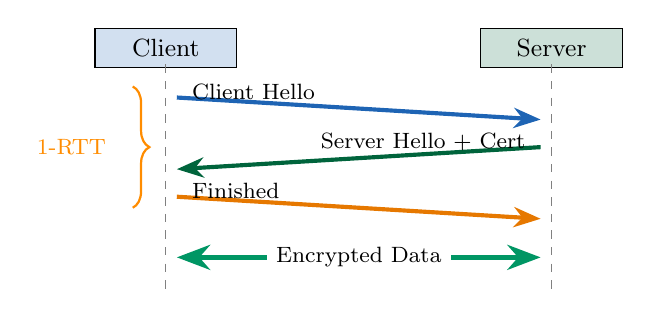
\begin{tikzpicture}[scale=0.7]
            % Client and Server columns
            \node[draw, fill=tcpblue!20, minimum width=1.8cm, minimum height=0.5cm, font=\small] (client) at (0, 4.5) {Client};
            \node[draw, fill=paddysgreen!20, minimum width=1.8cm, minimum height=0.5cm, font=\small] (server) at (7, 4.5) {Server};
            
            % Timeline
            \draw[dashed, gray] (0, 4.2) -- (0, 0);
            \draw[dashed, gray] (7, 4.2) -- (7, 0);
            
            % Step 1: Client Hello
            \draw[-{Stealth}, tcpblue, line width=1.5pt] (0.2, 3.6) -- (6.8, 3.2);
            \node[font=\footnotesize, right] at (0.3, 3.7) {Client Hello};
            
            % Step 2: Server Hello
            \draw[-{Stealth}, paddysgreen, line width=1.5pt] (6.8, 2.7) -- (0.2, 2.3);
            \node[font=\footnotesize, left] at (6.7, 2.8) {Server Hello + Cert};
            
            % Step 3: Finished
            \draw[-{Stealth}, aborange, line width=1.5pt] (0.2, 1.8) -- (6.8, 1.4);
            \node[font=\footnotesize, right] at (0.3, 1.9) {Finished};
            
            % Step 4: Application Data
            \draw[{Stealth}-{Stealth}, networkgreen, line width=2pt] (0.2, 0.7) -- (6.8, 0.7);
            \node[font=\footnotesize, fill=white] at (3.5, 0.7) {Encrypted Data};
            
            % Highlight: 1-RTT
            \draw[decorate, decoration={brace, amplitude=6pt}, thick, sunnyorange]
                (-0.6, 3.8) -- (-0.6, 1.6) node[midway, left=6pt, font=\footnotesize, sunnyorange] {1-RTT};
        \end{tikzpicture}
    \end{center}
    
    \begin{columns}[T]
        \begin{column}{0.48\textwidth}
            \begin{block}{TLS 1.3 Improvements}
                \footnotesize
                \begin{itemize}\setlength{\itemsep}{0pt}
                    \item 1-RTT handshake (faster than 1.2's 2-RTT)
                    \item 0-RTT resumption for repeat connections
                    \item Removed insecure cipher suites
                \end{itemize}
            \end{block}
        \end{column}
        \begin{column}{0.48\textwidth}
            \begin{alertblock}{Key Exchange}
                \footnotesize
                TLS 1.3 uses \textbf{Ephemeral Diffie-Hellman} exclusively---provides Perfect Forward Secrecy!
            \end{alertblock}
        \end{column}
    \end{columns}
\end{frame}

% =============================================================================
% SLIDE 7: TLS Certificates and Trust
% =============================================================================
\begin{frame}{TLS Certificates and Trust}
    \begin{columns}[T]
        \begin{column}{0.48\textwidth}
            \begin{block}{Certificate Chain}
                \small
                \begin{itemize}\setlength{\itemsep}{2pt}
                    \item \textbf{Root CA}: Pre-installed in browsers/OS
                    \item \textbf{Intermediate CA}: Signed by Root
                    \item \textbf{Server Certificate}: Signed by Intermediate
                \end{itemize}
            \end{block}
            
            \vspace{0.2em}
            \begin{block}{Certificate Fields}
                \small
                \begin{itemize}\setlength{\itemsep}{1pt}
                    \item \textbf{CN}: Common Name (domain)
                    \item \textbf{SAN}: Subject Alternative Names
                    \item \textbf{Validity}: Not Before / Not After dates
                    \item \textbf{Public Key}: For encryption
                    \item \textbf{Signature}: CA's digital signature
                \end{itemize}
            \end{block}
        \end{column}
        \begin{column}{0.48\textwidth}
            \begin{center}
                \begin{tikzpicture}[scale=0.7]
                    % Root CA
                    \node[draw=paddysgreen, fill=paddysgreen!20, rounded corners, 
                          minimum width=2.5cm, minimum height=0.7cm, font=\small] 
                          (root) at (0, 3) {Root CA};
                    \node[font=\tiny] at (0, 2.5) {\iconlock[0.25cm] Trusted};
                    
                    % Intermediate CA
                    \node[draw=tcpblue, fill=tcpblue!20, rounded corners, 
                          minimum width=2.5cm, minimum height=0.7cm, font=\small] 
                          (inter) at (0, 1.5) {Intermediate CA};
                    
                    % Server Cert
                    \node[draw=aborange, fill=aborange!20, rounded corners, 
                          minimum width=2.5cm, minimum height=0.7cm, font=\small] 
                          (server) at (0, 0) {Server Certificate};
                    \node[font=\tiny] at (0, -0.5) {\ttfamily www.example.com};
                    
                    % Arrows (signs)
                    \draw[-{Stealth}, paddysgreen, line width=1.5pt] (root) -- (inter) 
                        node[midway, right, font=\tiny] {signs};
                    \draw[-{Stealth}, tcpblue, line width=1.5pt] (inter) -- (server) 
                        node[midway, right, font=\tiny] {signs};
                \end{tikzpicture}
            \end{center}
            
            \vspace{0.3em}
            \begin{alertblock}{Self-Signed Certificates}
                \small
                Not trusted by browsers! Use for testing only. Production sites need CA-signed certificates (Let's Encrypt is free!).
            \end{alertblock}
        \end{column}
    \end{columns}
\end{frame}

% =============================================================================
% SLIDE 8: Network Time Protocol (NTP)
% =============================================================================
\begin{frame}{Network Time Protocol (NTP)}
    \begin{columns}[T]
        \begin{column}{0.48\textwidth}
            \begin{block}{NTP Basics}
                \small
                \begin{itemize}\setlength{\itemsep}{2pt}
                    \item \textbf{Port}: UDP 123
                    \item \textbf{Purpose}: Synchronize clocks across networks
                    \item \textbf{Accuracy}: Typically within milliseconds
                    \item \textbf{Polling}: Clients query servers periodically
                \end{itemize}
            \end{block}
            
            \vspace{0.2em}
            \begin{block}{Stratum Levels}
                \small
                \begin{itemize}\setlength{\itemsep}{1pt}
                    \item \textbf{Stratum 0}: Atomic clocks, GPS (reference)
                    \item \textbf{Stratum 1}: Directly connected to Stratum 0
                    \item \textbf{Stratum 2}: Syncs from Stratum 1
                    \item \textbf{Stratum 3+}: Each level adds latency
                \end{itemize}
            \end{block}
        \end{column}
        \begin{column}{0.48\textwidth}
            \begin{center}
                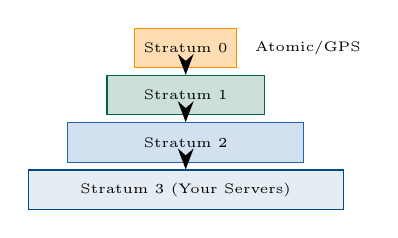
\begin{tikzpicture}[scale=0.6]
                    % Stratum pyramid
                    \node[draw=sunnyorange, fill=sunnyorange!30, minimum width=1cm, 
                          minimum height=0.5cm, font=\tiny] (s0) at (0, 3) {Stratum 0};
                    \node[font=\tiny, right=0.1cm of s0] {Atomic/GPS};
                    
                    \node[draw=paddysgreen, fill=paddysgreen!20, minimum width=2cm, 
                          minimum height=0.5cm, font=\tiny] (s1) at (0, 2) {Stratum 1};
                    
                    \node[draw=tcpblue, fill=tcpblue!20, minimum width=3cm, 
                          minimum height=0.5cm, font=\tiny] (s2) at (0, 1) {Stratum 2};
                    
                    \node[draw=rctcblue, fill=rctcblue!10, minimum width=4cm, 
                          minimum height=0.5cm, font=\tiny] (s3) at (0, 0) {Stratum 3 (Your Servers)};
                    
                    % Arrows
                    \draw[-{Stealth}, line width=1pt] (s0) -- (s1);
                    \draw[-{Stealth}, line width=1pt] (s1) -- (s2);
                    \draw[-{Stealth}, line width=1pt] (s2) -- (s3);
                \end{tikzpicture}
            \end{center}
            
            \vspace{0.3em}
            \begin{exampleblock}{Public NTP Servers}
                \small
                \ttfamily
                pool.ntp.org \\
                time.google.com \\
                time.nist.gov \\
                time.windows.com
            \end{exampleblock}
        \end{column}
    \end{columns}
\end{frame}

% =============================================================================
% SLIDE 9: NTP Architecture and Synchronization
% =============================================================================
\begin{frame}{NTP Architecture and Configuration}
    \begin{columns}[T]
        \begin{column}{0.48\textwidth}
            \begin{center}
                \begin{tikzpicture}[scale=0.55]
                    % NTP Pool
                    \node[cloud, draw=tcpblue, fill=tcpblue!10] (pool) at (0, 2.8) {\iconcloud[0.4cm]};
                    \node[font=\tiny] at (0, 2.3) {NTP Pool};
                    
                    % Local NTP Server
                    \node[server] (local) at (0, 1) {\iconserver[0.4cm]};
                    \node[font=\tiny] at (0, 0.5) {Local NTP};
                    
                    % Clients
                    \node[pc] (c1) at (-1.8, -0.7) {\iconpc[0.3cm]};
                    \node[pc] (c2) at (0, -0.7) {\iconpc[0.3cm]};
                    \node[pc] (c3) at (1.8, -0.7) {\iconpc[0.3cm]};
                    
                    % Connections
                    \draw[-{Stealth}, udpgreen, line width=1pt] (pool) -- (local) 
                        node[midway, right, font=\tiny] {UDP 123};
                    \draw[-{Stealth}, line width=0.8pt] (local) -- (c1);
                    \draw[-{Stealth}, line width=0.8pt] (local) -- (c2);
                    \draw[-{Stealth}, line width=0.8pt] (local) -- (c3);
                \end{tikzpicture}
            \end{center}
            
            \begin{alertblock}{Why Local NTP Server?}
                \footnotesize
                Reduces external traffic, provides consistent time if internet fails.
            \end{alertblock}
        \end{column}
        \begin{column}{0.48\textwidth}
            \begin{block}{Linux NTP Configuration}
                \ttfamily\scriptsize
                \# /etc/chrony/chrony.conf \\
                server pool.ntp.org iburst \\
                server time.google.com iburst
            \end{block}
            
            \begin{block}{Useful Commands}
                \ttfamily\scriptsize
                timedatectl status \\
                chronyc sources -v \\
                chronyc tracking
            \end{block}
            
            \begin{exampleblock}{Kerberos Requirement}
                \footnotesize
                Kerberos requires clocks within \textbf{5 minutes}---NTP is essential for AD!
            \end{exampleblock}
        \end{column}
    \end{columns}
\end{frame}

% =============================================================================
% SLIDE 10: Precision Time Protocol (PTP)
% =============================================================================
\begin{frame}{Precision Time Protocol (PTP)}
    \begin{columns}[T]
        \begin{column}{0.48\textwidth}
            \begin{block}{PTP Overview}
                \small
                \begin{itemize}\setlength{\itemsep}{2pt}
                    \item \textbf{Standard}: IEEE 1588
                    \item \textbf{Ports}: UDP 319 (event), 320 (general)
                    \item \textbf{Accuracy}: Sub-microsecond to nanoseconds
                    \item \textbf{Requirement}: Hardware timestamping support
                \end{itemize}
            \end{block}
            
            \vspace{0.2em}
            \begin{block}{PTP Use Cases}
                \small
                \begin{itemize}\setlength{\itemsep}{1pt}
                    \item Financial trading (timestamps matter!)
                    \item Telecommunications (5G networks)
                    \item Industrial automation
                    \item Broadcast media synchronization
                \end{itemize}
            \end{block}
        \end{column}
        \begin{column}{0.48\textwidth}
            \begin{block}{NTP vs PTP Comparison}
                \small
                \begin{tabular}{@{}l c c@{}}
                    \toprule
                    \textbf{Feature} & \textbf{NTP} & \textbf{PTP} \\
                    \midrule
                    Accuracy & ms & ns--$\mu$s \\
                    Port & UDP 123 & UDP 319/320 \\
                    Hardware & Software & HW assist \\
                    Cost & Low & Higher \\
                    Complexity & Simple & Complex \\
                    Use Case & General & Precision \\
                    \bottomrule
                \end{tabular}
            \end{block}
            
            \vspace{0.3em}
            \begin{alertblock}{When to Use PTP}
                \small
                Only needed when \textbf{microsecond accuracy} is required. For most networks, NTP is sufficient and simpler!
            \end{alertblock}
        \end{column}
    \end{columns}
\end{frame}

% =============================================================================
% SLIDE 11: Case Study - Dennis & The Paddy's Time Heist
% =============================================================================
\begin{frame}{Case Study: Dennis \& The Paddy's Time Heist}
    \begin{casestudy}{``The Gang's POS System Fails''}
        \small
        Dennis notices Paddy's Pub POS system is suddenly rejecting all credit card transactions. The error message reads: \textbf{``Certificate not yet valid.''}
        
        \vspace{0.3em}
        Upon investigation, Dennis sees the system clock shows \textbf{January 15, 2019} instead of the current date. Mac admits he ``fixed'' the server by unplugging it during a storm last week and never bothered to check if it came back up properly.
        
        \vspace{0.3em}
        \ttfamily\footnotesize
        \begin{tabular}{l l}
            System Time: & 2019-01-15 14:32:00 \\
            Certificate Valid: & 2023-06-01 to 2025-06-01 \\
            Error: & SSL\_ERROR\_FUTURE\_CERT \\
        \end{tabular}
    \end{casestudy}
    
    \begin{block}{Review Questions}
        \small
        \begin{enumerate}\setlength{\itemsep}{1pt}
            \item Why are TLS certificates failing validation?
            \item What protocol should be configured to prevent this?
            \item How would you immediately fix this issue?
        \end{enumerate}
    \end{block}
\end{frame}

% =============================================================================
% SLIDE 12: Case Study Solution - Dennis & The Paddy's Time Heist
% =============================================================================
\begin{frame}{Case Study Solution: Dennis \& The Paddy's Time Heist}
    \begin{casesolution}{``The Gang Learns About Time Sync''}
        \small
        \begin{enumerate}\setlength{\itemsep}{2pt}
            \item System clock is in the \textbf{past} (2019), so certificates issued in 2023 appear ``not yet valid''---the system thinks it's before the certificate start date!
            \item Configure \textbf{NTP} to automatically synchronize with reliable time servers
            \item \textbf{Immediate fix}: Manually set time or enable NTP sync
        \end{enumerate}
    \end{casesolution}
    
    \begin{columns}[T]
        \begin{column}{0.48\textwidth}
            \begin{block}{Quick Fix Commands}
                \ttfamily\small
                \# Check current status \\
                timedatectl status \\[0.3em]
                \# Enable NTP sync \\
                sudo timedatectl set-ntp true \\[0.3em]
                \# Or use chronyd \\
                sudo systemctl enable chronyd \\
                sudo systemctl start chronyd
            \end{block}
        \end{column}
        \begin{column}{0.48\textwidth}
            \begin{alertblock}{Key Lesson}
                \small
                ``It's not just about the money, it's about sending a message... to the NTP server.'' 
                
                \vspace{0.2em}
                \normalfont Certificates, Kerberos, logs, and scheduled tasks \textbf{all depend on accurate time!}
            \end{alertblock}
        \end{column}
    \end{columns}
\end{frame}

% =============================================================================
% SLIDE 15: HTTP - Hypertext Transfer Protocol
% =============================================================================
\begin{frame}{HTTP --- Hypertext Transfer Protocol}
    \begin{columns}[T]
        \begin{column}{0.48\textwidth}
            \begin{block}{HTTP Basics}
                \footnotesize
                \begin{itemize}\setlength{\itemsep}{1pt}
                    \item \textbf{Port}: TCP 80 (unencrypted!)
                    \item \textbf{Model}: Request-Response
                    \item \textbf{Stateless}: Each request is independent
                    \item Cookies/sessions add state
                \end{itemize}
            \end{block}
            
            \begin{block}{HTTP Methods}
                \footnotesize
                \begin{itemize}\setlength{\itemsep}{0pt}
                    \item \textbf{GET}: Retrieve resource
                    \item \textbf{POST}: Submit data
                    \item \textbf{PUT}: Update/replace
                    \item \textbf{DELETE}: Remove resource
                \end{itemize}
            \end{block}
        \end{column}
        \begin{column}{0.48\textwidth}
            \begin{block}{HTTP Status Codes}
                \footnotesize
                \begin{tabular}{@{}c l@{}}
                    \toprule
                    \textbf{Code} & \textbf{Meaning} \\
                    \midrule
                    200 & OK \\
                    301 & Moved Permanently \\
                    400 & Bad Request \\
                    401 & Unauthorized \\
                    403 & Forbidden \\
                    404 & Not Found \\
                    500 & Server Error \\
                    \bottomrule
                \end{tabular}
            \end{block}
            
            \begin{alertblock}{Security Warning}
                \footnotesize
                HTTP sends everything in \textbf{cleartext}. Never use for sensitive info!
            \end{alertblock}
        \end{column}
    \end{columns}
\end{frame}

% =============================================================================
% SLIDE 16: HTTP/2 and HTTP/3
% =============================================================================
\begin{frame}{HTTP/2 and HTTP/3}
    \begin{columns}[T]
        \begin{column}{0.54\textwidth}
            \begin{block}{HTTP Version Comparison}
                \footnotesize
                \begin{tabular}{@{}l c c c@{}}
                    \toprule
                    \textbf{Feature} & \textbf{1.1} & \textbf{2} & \textbf{3} \\
                    \midrule
                    Transport & TCP & TCP & QUIC \\
                    Multiplex & No & Yes & Yes \\
                    Header Comp & No & HPACK & QPACK \\
                    Server Push & No & Yes & Yes \\
                    \bottomrule
                
                \end{tabular}
            \end{block}
            
            \vspace{0.2em}
            \begin{exampleblock}{HTTP/3 and QUIC}
                \small
                HTTP/3 uses \textbf{QUIC} (UDP-based) instead of TCP. Benefits: faster connection setup, better mobile performance, built-in encryption.
            \end{exampleblock}
        \end{column}
        \begin{column}{0.42\textwidth}
            \begin{center}
                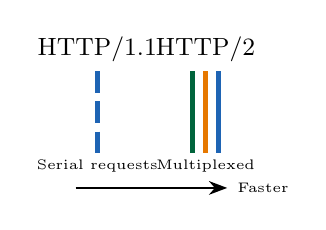
\begin{tikzpicture}[scale=0.55]
                    % HTTP/1.1 - serial
                    \node[font=\small, align=center] at (0, 3.5) {HTTP/1.1};
                    \draw[tcpblue, line width=2pt] (0, 3) -- (0, 2.5);
                    \draw[tcpblue, line width=2pt] (0, 2.3) -- (0, 1.8);
                    \draw[tcpblue, line width=2pt] (0, 1.6) -- (0, 1.1);
                    \node[font=\tiny] at (0, 0.8) {Serial requests};
                    
                    % HTTP/2 - multiplexed
                    \node[font=\small, align=center] at (2.5, 3.5) {HTTP/2};
                    \draw[paddysgreen, line width=2pt] (2.2, 3) -- (2.2, 1.1);
                    \draw[aborange, line width=2pt] (2.5, 3) -- (2.5, 1.1);
                    \draw[tcpblue, line width=2pt] (2.8, 3) -- (2.8, 1.1);
                    \node[font=\tiny] at (2.5, 0.8) {Multiplexed};
                    
                    % Arrows showing speed
                    \draw[-{Stealth}, thick] (-0.5, 0.3) -- (3, 0.3) node[right, font=\tiny] {Faster};
                \end{tikzpicture}
            \end{center}
            
            \vspace{0.2em}
            \begin{alertblock}{Key Takeaway}
                \small
                HTTP/2+ eliminates \textbf{head-of-line blocking}---multiple requests over single connection!
            \end{alertblock}
        \end{column}
    \end{columns}
\end{frame}

% =============================================================================
% SLIDE 17: HTTPS - HTTP Secure
% =============================================================================
\begin{frame}{HTTPS --- HTTP Secure}
    \begin{columns}[T]
        \begin{column}{0.48\textwidth}
            \begin{block}{HTTPS = HTTP + TLS}
                \small
                \begin{itemize}\setlength{\itemsep}{2pt}
                    \item \textbf{Port}: TCP 443
                    \item All HTTP traffic encrypted via TLS
                    \item Server authenticated via certificate
                    \item Data integrity protected
                \end{itemize}
            \end{block}
            
            \vspace{0.2em}
            \begin{block}{HSTS (HTTP Strict Transport Security)}
                \small
                Server header that forces browsers to \textbf{only use HTTPS}:
                
                \vspace{0.2em}
                \ttfamily\footnotesize
                Strict-Transport-Security: \\
                \ \ max-age=31536000; includeSubDomains
            \end{block}
        \end{column}
        \begin{column}{0.48\textwidth}
            \begin{center}
                \begin{tikzpicture}[scale=0.6]
                    % Browser
                    \node[pc] (browser) at (0, 2) {\iconpc[0.5cm]};
                    \node[font=\tiny] at (0, 1.4) {Browser};
                    
                    % Lock
                    \node (lock) at (2, 2) {\iconlock[0.4cm]};
                    
                    % Server
                    \node[server] (server) at (4, 2) {\iconserver[0.5cm]};
                    \node[font=\tiny] at (4, 1.4) {Web Server};
                    
                    % Certificate
                    \node[draw=paddysgreen, fill=paddysgreen!10, rounded corners, 
                          font=\tiny, text width=1.5cm, align=center] (cert) at (4, 0.3) 
                          {Certificate\\(443)};
                    
                    % Connections
                    \draw[secure, line width=1.5pt] (browser) -- (lock);
                    \draw[secure, line width=1.5pt] (lock) -- (server);
                    \draw[-{Stealth}, dashed] (server) -- (cert);
                \end{tikzpicture}
            \end{center}
            
            \vspace{0.3em}
            \begin{alertblock}{Verify Both!}
                \small
                Always check:
                \begin{itemize}\setlength{\itemsep}{0pt}
                    \item \iconlock[0.3cm] Padlock icon (encrypted)
                    \item Domain name matches expected site
                \end{itemize}
                Phishing sites can have valid certificates!
            \end{alertblock}
        \end{column}
    \end{columns}
\end{frame}

% =============================================================================
% SLIDE 18: FTP - File Transfer Protocol
% =============================================================================
\begin{frame}{FTP --- File Transfer Protocol}
    \begin{columns}[T]
        \begin{column}{0.48\textwidth}
            \begin{block}{FTP Basics}
                \footnotesize
                \begin{itemize}\setlength{\itemsep}{1pt}
                    \item \textbf{Control}: TCP port 21
                    \item \textbf{Data}: TCP port 20 (active mode)
                    \item Two separate connections
                    \item \textcolor{alertred}{Cleartext credentials!}
                \end{itemize}
            \end{block}
            
            \begin{block}{FTP Modes}
                \footnotesize
                \textbf{Active}: Server connects TO client for data; \textcolor{alertred}{blocked by firewalls}
                
                \vspace{0.1em}
                \textbf{Passive (PASV)}: Client connects TO server; \textcolor{paddysgreen}{firewall-friendly}
            \end{block}
        \end{column}
        \begin{column}{0.48\textwidth}
            \begin{center}
                \begin{tikzpicture}[scale=0.5]
                    % Active mode
                    \node[font=\footnotesize] at (0, 3.2) {\textbf{Active Mode}};
                    \node[pc] (c1) at (-1.5, 2.3) {\iconpc[0.35cm]};
                    \node[server] (s1) at (1.5, 2.3) {\iconserver[0.35cm]};
                    \draw[-{Stealth}, tcpblue] (c1) -- (s1) node[midway, above, font=\tiny] {21};
                    \draw[-{Stealth}, alertred] (s1) to[bend right=20] node[midway, below, font=\tiny] {20→Client} (c1);
                    
                    % Passive mode
                    \node[font=\footnotesize] at (0, 0.8) {\textbf{Passive Mode}};
                    \node[pc] (c2) at (-1.5, -0.1) {\iconpc[0.35cm]};
                    \node[server] (s2) at (1.5, -0.1) {\iconserver[0.35cm]};
                    \draw[-{Stealth}, tcpblue] (c2) -- (s2) node[midway, above, font=\tiny] {21};
                    \draw[-{Stealth}, paddysgreen] (c2) to[bend right=20] node[midway, below, font=\tiny] {→High Port} (s2);
                \end{tikzpicture}
            \end{center}
            
            \begin{alertblock}{Security Warning}
                \footnotesize
                FTP sends credentials in \textbf{cleartext}. Use SFTP or FTPS instead!
            \end{alertblock}
        \end{column}
    \end{columns}
\end{frame}

% =============================================================================
% SLIDE 19: Secure File Transfer - SFTP, FTPS, SCP
% =============================================================================
\begin{frame}{Secure File Transfer: SFTP, FTPS, and SCP}
    \begin{block}{Secure File Transfer Comparison}
        \footnotesize
        \begin{tabular}{@{}l c c c l@{}}
            \toprule
            \textbf{Protocol} & \textbf{Port(s)} & \textbf{Encryption} & \textbf{Based On} & \textbf{Notes} \\
            \midrule
            \textbf{SFTP} & 22 & SSH & SSH subsystem & Single connection \\
            \textbf{FTPS} & 989/990 & TLS & FTP + TLS & Explicit or Implicit \\
            \textbf{SCP} & 22 & SSH & SSH/RCP & Simple copy only \\
            \textbf{FTP} & 20/21 & \textcolor{alertred}{None} & --- & \textcolor{alertred}{Insecure} \\
            \bottomrule
        \end{tabular}
    \end{block}
    
    \begin{columns}[T]
        \begin{column}{0.48\textwidth}
            \begin{exampleblock}{SFTP (Recommended)}
                \footnotesize
                \begin{itemize}\setlength{\itemsep}{0pt}
                    \item Uses SSH infrastructure (port 22)
                    \item Single encrypted connection
                    \item Full file operations
                    \item Key-based auth supported
                \end{itemize}
                \ttfamily\scriptsize
                sftp user@server.com
            \end{exampleblock}
        \end{column}
        \begin{column}{0.48\textwidth}
            \begin{block}{FTPS Modes}
                \footnotesize
                \textbf{Explicit}: Start plain, upgrade via STARTTLS (port 21)
                
                \textbf{Implicit}: TLS from start (port 990)
            \end{block}
            
            \begin{alertblock}{Firewall Note}
                \footnotesize
                FTPS still uses separate data connections. SFTP is simpler!
            \end{alertblock}
        \end{column}
    \end{columns}
\end{frame}

% =============================================================================
% SLIDE 20: SMB - Server Message Block
% =============================================================================
\begin{frame}{SMB --- Server Message Block}
    \begin{columns}[T]
        \begin{column}{0.48\textwidth}
            \begin{block}{SMB Overview}
                \small
                \begin{itemize}\setlength{\itemsep}{2pt}
                    \item Windows file and print sharing
                    \item \textbf{Port}: TCP 445 (direct)
                    \item Legacy: TCP 137--139 (NetBIOS)
                    \item UNC paths: \texttt{\textbackslash\textbackslash server\textbackslash share}
                \end{itemize}
            \end{block}
            
            \vspace{0.2em}
            \begin{block}{SMB Versions}
                \small
                \begin{itemize}\setlength{\itemsep}{1pt}
                    \item \textbf{SMB1}: \textcolor{alertred}{Vulnerable! Disable it!}
                    \item \textbf{SMB2}: Windows Vista/2008+
                    \item \textbf{SMB2.1}: Windows 7/2008 R2
                    \item \textbf{SMB3}: Windows 8/2012+ (encryption)
                    \item \textbf{SMB3.1.1}: Windows 10/2016+ (pre-auth integrity)
                \end{itemize}
            \end{block}
        \end{column}
        \begin{column}{0.48\textwidth}
            \begin{center}
                \begin{tikzpicture}[scale=0.6]
                    % File Server
                    \node[server] (server) at (0, 2) {\iconserver[0.6cm]};
                    \node[font=\tiny] at (0, 1.3) {File Server};
                    \node[font=\tiny, tcpblue] at (0, 0.9) {TCP 445};
                    
                    % Clients
                    \node[pc] (c1) at (-2, 0) {\iconpc[0.4cm]};
                    \node[pc] (c2) at (0, -0.5) {\iconpc[0.4cm]};
                    \node[pc] (c3) at (2, 0) {\iconpc[0.4cm]};
                    
                    % Connections
                    \draw[ethernet] (c1) -- (server);
                    \draw[ethernet] (c2) -- (server);
                    \draw[ethernet] (c3) -- (server);
                    
                    % Share label
                    \node[draw, fill=rctcblue!10, rounded corners, font=\tiny] at (0, 3) 
                          {\texttt{\textbackslash\textbackslash FileServer\textbackslash Shared}};
                \end{tikzpicture}
            \end{center}
            
            \vspace{0.2em}
            \begin{alertblock}{CRITICAL: Disable SMB1!}
                \small
                SMB1 is vulnerable to \textbf{EternalBlue} exploit (WannaCry, NotPetya). Disable via:
                
                {\ttfamily\footnotesize
                Disable-WindowsOptionalFeature\newline
                \ \ -FeatureName SMB1Protocol}
            \end{alertblock}
        \end{column}
    \end{columns}
\end{frame}

% =============================================================================
% SLIDE 21: Network Attached Storage (NAS)
% =============================================================================
\begin{frame}{Network Attached Storage (NAS)}
    \begin{columns}[T]
        \begin{column}{0.48\textwidth}
            \begin{block}{NAS Overview}
                \small
                \begin{itemize}\setlength{\itemsep}{2pt}
                    \item \textbf{File-level} storage over network
                    \item Dedicated storage appliance
                    \item Protocols: SMB, NFS, AFP
                    \item Easy setup and management
                    \item Good for SMB (small-medium business)
                \end{itemize}
            \end{block}
            
            \vspace{0.2em}
            \begin{block}{Common NAS Protocols}
                \small
                \begin{itemize}\setlength{\itemsep}{1pt}
                    \item \textbf{SMB/CIFS}: Windows clients
                    \item \textbf{NFS}: Linux/Unix clients (TCP 2049)
                    \item \textbf{AFP}: Legacy Mac (TCP 548)
                    \item \textbf{iSCSI}: Block-level (acts like SAN)
                \end{itemize}
            \end{block}
        \end{column}
        \begin{column}{0.48\textwidth}
            \begin{block}{NAS vs SAN}
                \small
                \begin{tabular}{@{}l c c@{}}
                    \toprule
                    & \textbf{NAS} & \textbf{SAN} \\
                    \midrule
                    Storage Level & File & Block \\
                    Protocol & SMB/NFS & FC/iSCSI \\
                    Network & Ethernet & Dedicated \\
                    Complexity & Low & High \\
                    Cost & \$ & \$\$\$ \\
                    Best For & File sharing & Databases \\
                    \bottomrule
                \end{tabular}
            \end{block}
            
            \vspace{0.2em}
            \begin{center}
                \begin{tikzpicture}[scale=0.5]
                    % NAS
                    \node[draw=tcpblue, fill=tcpblue!10, rounded corners, 
                          minimum width=1.5cm, minimum height=1cm] (nas) at (0,0) 
                          {\icondatabase[0.4cm]};
                    \node[font=\tiny] at (0, -0.8) {NAS};
                    
                    % Clients
                    \node[pc] (c1) at (-2, 0.5) {\iconpc[0.3cm]};
                    \node[pc] (c2) at (-2, -0.5) {\iconpc[0.3cm]};
                    \node[laptop] (c3) at (2, 0) {\iconlaptop[0.3cm]};
                    
                    % Connections
                    \draw[ethernet noarrow] (c1) -- (nas);
                    \draw[ethernet noarrow] (c2) -- (nas);
                    \draw[ethernet noarrow] (c3) -- (nas);
                \end{tikzpicture}
            \end{center}
        \end{column}
    \end{columns}
\end{frame}

% =============================================================================
% SLIDE 22: Database Services
% =============================================================================
\begin{frame}{Database Services}
    \begin{columns}[T]
        \begin{column}{0.48\textwidth}
            \begin{block}{Common Database Ports}
                \small
                \begin{tabular}{@{}l c l@{}}
                    \toprule
                    \textbf{Database} & \textbf{Port} & \textbf{Type} \\
                    \midrule
                    MySQL/MariaDB & 3306 & SQL \\
                    PostgreSQL & 5432 & SQL \\
                    MS SQL Server & 1433 & SQL \\
                    Oracle & 1521 & SQL \\
                    MongoDB & 27017 & NoSQL \\
                    Redis & 6379 & NoSQL/Cache \\
                    \bottomrule
                \end{tabular}
            \end{block}
            
            \vspace{0.2em}
            \begin{block}{Database Connectivity}
                \small
                \begin{itemize}\setlength{\itemsep}{1pt}
                    \item \textbf{ODBC}: Open Database Connectivity (Windows)
                    \item \textbf{JDBC}: Java Database Connectivity
                    \item Native drivers for each database
                \end{itemize}
            \end{block}
        \end{column}
        \begin{column}{0.48\textwidth}
            \begin{center}
                \begin{tikzpicture}[scale=0.55]
                    % Three-tier architecture
                    % Client tier
                    \node[pc] (client) at (0, 3) {\iconpc[0.5cm]};
                    \node[font=\tiny] at (0, 2.4) {Client};
                    
                    % Web/App tier
                    \node[server] (web) at (0, 1.5) {\iconserver[0.5cm]};
                    \node[font=\tiny] at (0, 0.9) {Web/App Server};
                    
                    % Database tier
                    \node (db) at (0, 0) {\icondatabase[0.5cm]};
                    \node[font=\tiny] at (0, -0.6) {Database};
                    
                    % Connections
                    \draw[-{Stealth}, tcpblue, line width=1pt] (client) -- (web) 
                        node[midway, right, font=\tiny] {HTTP(S)};
                    \draw[-{Stealth}, paddysgreen, line width=1pt] (web) -- (db) 
                        node[midway, right, font=\tiny] {SQL};
                    
                    % Labels
                    \node[font=\tiny, gray] at (2, 3) {Presentation};
                    \node[font=\tiny, gray] at (2, 1.5) {Application};
                    \node[font=\tiny, gray] at (2, 0) {Data};
                \end{tikzpicture}
            \end{center}
            
            \vspace{0.2em}
            \begin{alertblock}{Security Best Practices}
                \small
                \begin{itemize}\setlength{\itemsep}{0pt}
                    \item Never expose DB directly to internet
                    \item Use firewall rules to restrict access
                    \item Encrypt connections (TLS)
                    \item Use least-privilege accounts
                \end{itemize}
            \end{alertblock}
        \end{column}
    \end{columns}
\end{frame}

% =============================================================================
% SLIDE 23: Case Study - Charlie's Rat Business Website
% =============================================================================
\begin{frame}{Case Study: Charlie's Rat Business Website}
    \begin{casestudy}{``Charlie's Rat Removal Goes Online''}
        \small
        Charlie has created a website for his new business ``Charlie's Rat Removal \& Bird Law Consulting'' using plain HTTP on port 80.
        
        \vspace{0.3em}
        Frank wants to add online payment processing to collect service fees. However, customers are complaining that their browsers display \textbf{``Not Secure''} warnings.
        
        \vspace{0.3em}
        Charlie insists: ``But it works fine on my computer! The rats don't care about security!''
        
        \vspace{0.3em}
        \ttfamily\footnotesize
        \begin{tabular}{l l}
            Current URL: & http://charliesratremoval.com \\
            Port: & TCP 80 \\
            Browser Warning: & ``Not Secure'' \\
            Payment Processor: & Refuses to integrate \\
        \end{tabular}
    \end{casestudy}
    
    \begin{block}{Review Questions}
        \small
        \begin{enumerate}\setlength{\itemsep}{1pt}
            \item What is the security risk of using plain HTTP?
            \item What needs to be implemented to fix this?
            \item What port and protocol changes are needed?
        \end{enumerate}
    \end{block}
\end{frame}

% =============================================================================
% SLIDE 24: Case Study Solution - Charlie's Rat Business Website
% =============================================================================
\begin{frame}{Case Study Solution: Charlie's Rat Business Website}
    \begin{casesolution}{``Charlie Learns HTTPS''}
        \small
        \begin{enumerate}\setlength{\itemsep}{2pt}
            \item HTTP transmits \textbf{everything in cleartext}---including payment info, passwords, and customer data. Anyone on the network can intercept it!
            \item Implement \textbf{HTTPS} with a valid TLS certificate. Let's Encrypt provides free certificates!
            \item Change from port \textbf{80 to 443}, configure TLS, and set up HTTP→HTTPS redirect.
        \end{enumerate}
    \end{casesolution}
    
    \begin{columns}[T]
        \begin{column}{0.48\textwidth}
            \begin{block}{Apache HTTPS Redirect}
                \ttfamily\footnotesize
                <VirtualHost *:80> \\
                \ \ ServerName charliesratremoval.com \\
                \ \ Redirect permanent / \\
                \ \ \ \ https://charliesratremoval.com/ \\
                </VirtualHost>
            \end{block}
        \end{column}
        \begin{column}{0.48\textwidth}
            \begin{alertblock}{Key Lesson}
                \small
                ``The rats may not care, but PCI-DSS does!''
                
                \vspace{0.2em}
                \normalfont Payment Card Industry compliance \textbf{requires encryption}. No HTTPS = no payment processing!
            \end{alertblock}
        \end{column}
    \end{columns}
\end{frame}

% =============================================================================
% SLIDE 27: Email Architecture Overview
% =============================================================================
\begin{frame}{Email Architecture Overview}
    \begin{center}
        \begin{tikzpicture}[scale=0.7]
            % Sender side
            \node[pc] (sender) at (0, 0) {\iconpc[0.5cm]};
            \node[font=\tiny, below=0.1cm of sender] {Sender (MUA)};
            
            % Sender's mail server
            \node[server] (msa) at (3, 0) {\iconserver[0.5cm]};
            \node[font=\tiny, below=0.1cm of msa] {MSA/MTA};
            
            % Internet
            \node[cloud] (internet) at (6, 0) {\iconcloud[0.6cm]};
            \node[font=\tiny, below=0.1cm of internet] {Internet};
            
            % Recipient's mail server
            \node[server] (mda) at (9, 0) {\iconserver[0.5cm]};
            \node[font=\tiny, below=0.1cm of mda] {MTA/MDA};
            
            % Recipient
            \node[pc] (receiver) at (12, 0) {\iconpc[0.5cm]};
            \node[font=\tiny, below=0.1cm of receiver] {Recipient (MUA)};
            
            % Connections with labels
            \draw[-{Stealth}, tcpblue, line width=1.5pt] (sender) -- (msa) 
                node[midway, above, font=\tiny] {SMTP (587)};
            \draw[-{Stealth}, tcpblue, line width=1.5pt] (msa) -- (internet) 
                node[midway, above, font=\tiny] {SMTP (25)};
            \draw[-{Stealth}, tcpblue, line width=1.5pt] (internet) -- (mda) 
                node[midway, above, font=\tiny] {SMTP (25)};
            \draw[-{Stealth}, paddysgreen, line width=1.5pt] (mda) -- (receiver) 
                node[midway, above, font=\tiny] {IMAP/POP3};
        \end{tikzpicture}
    \end{center}
    
    \begin{columns}[T]
        \begin{column}{0.48\textwidth}
            \begin{block}{Email Components}
                \small
                \begin{itemize}\setlength{\itemsep}{1pt}
                    \item \textbf{MUA}: Mail User Agent (client app)
                    \item \textbf{MSA}: Mail Submission Agent
                    \item \textbf{MTA}: Mail Transfer Agent (server-to-server)
                    \item \textbf{MDA}: Mail Delivery Agent (to mailbox)
                \end{itemize}
            \end{block}
        \end{column}
        \begin{column}{0.48\textwidth}
            \begin{exampleblock}{Store-and-Forward}
                \small
                Email uses \textbf{store-and-forward}: each server receives the message, stores it, then forwards to the next hop. Unlike real-time communication!
            \end{exampleblock}
        \end{column}
    \end{columns}
\end{frame}

% =============================================================================
% SLIDE 28: SMTP - Simple Mail Transfer Protocol
% =============================================================================
\begin{frame}{SMTP --- Simple Mail Transfer Protocol}
    \begin{columns}[T]
        \begin{column}{0.48\textwidth}
            \begin{block}{SMTP Basics}
                \small
                \begin{itemize}\setlength{\itemsep}{2pt}
                    \item \textbf{Port 25}: Server-to-server (MTA)
                    \item \textbf{Port 587}: Client submission (MSA)
                    \item \textbf{Port 465}: SMTPS (implicit TLS)
                    \item \textbf{STARTTLS}: Upgrade to encrypted
                    \item \textbf{Push protocol}: Sending only!
                \end{itemize}
            \end{block}
            
            \vspace{0.2em}
            \begin{block}{Email Authentication}
                \small
                \begin{itemize}\setlength{\itemsep}{1pt}
                    \item \textbf{SPF}: Authorized senders (DNS TXT)
                    \item \textbf{DKIM}: Digital signature
                    \item \textbf{DMARC}: Policy enforcement
                \end{itemize}
                Prevents spoofing and phishing!
            \end{block}
        \end{column}
        \begin{column}{0.48\textwidth}
            \begin{block}{SMTP Session Example}
                \ttfamily\footnotesize
                S: 220 mail.example.com SMTP \\
                C: HELO client.com \\
                S: 250 Hello client.com \\
                C: MAIL FROM:<sender@client.com> \\
                S: 250 OK \\
                C: RCPT TO:<user@example.com> \\
                S: 250 OK \\
                C: DATA \\
                S: 354 Start mail input \\
                C: Subject: Test \\
                C: \\
                C: Message body here. \\
                C: . \\
                S: 250 OK \\
                C: QUIT
            \end{block}
        \end{column}
    \end{columns}
\end{frame}

% =============================================================================
% SLIDE 29: IMAP and POP3 - Receiving Email
% =============================================================================
\begin{frame}{IMAP and POP3 --- Receiving Email}
    \begin{columns}[T]
        \begin{column}{0.55\textwidth}
            \begin{block}{IMAP vs POP3 Comparison}
                \small
                \begin{tabular}{@{}l c c@{}}
                    \toprule
                    \textbf{Feature} & \textbf{IMAP} & \textbf{POP3} \\
                    \midrule
                    Port (plain) & 143 & 110 \\
                    Port (TLS) & 993 & 995 \\
                    Mail Storage & Server & Downloads \\
                    Multi-device & \textcolor{paddysgreen}{Yes} & \textcolor{alertred}{Limited} \\
                    Folders & \textcolor{paddysgreen}{Synced} & \textcolor{alertred}{Local only} \\
                    Bandwidth & Higher & Lower \\
                    Offline & Sync folders & Full access \\
                    Server Space & Uses more & Uses less \\
                    \bottomrule
                \end{tabular}
            \end{block}
        \end{column}
        \begin{column}{0.42\textwidth}
            \begin{center}
                \begin{tikzpicture}[scale=0.5]
                    % IMAP
                    \node[font=\small] at (0, 3) {\textbf{IMAP}};
                    \node[server] (s1) at (0, 2) {\iconserver[0.4cm]};
                    \node[pc] (c1a) at (-1, 0.5) {\iconpc[0.3cm]};
                    \node[laptop] (c1b) at (1, 0.5) {\iconlaptop[0.3cm]};
                    \draw[{Stealth}-{Stealth}, paddysgreen] (s1) -- (c1a);
                    \draw[{Stealth}-{Stealth}, paddysgreen] (s1) -- (c1b);
                    \node[font=\tiny] at (0, -0.2) {Mail stays on server};
                    
                    % POP3
                    \node[font=\small] at (4, 3) {\textbf{POP3}};
                    \node[server] (s2) at (4, 2) {\iconserver[0.4cm]};
                    \node[pc] (c2) at (4, 0.5) {\iconpc[0.4cm]};
                    \draw[-{Stealth}, aborange, line width=1.5pt] (s2) -- (c2);
                    \node[font=\tiny] at (4, -0.2) {Downloads to client};
                \end{tikzpicture}
            \end{center}
            
            \vspace{0.2em}
            \begin{exampleblock}{When to Use}
                \small
                \textbf{IMAP}: Multiple devices, mobile users
                
                \textbf{POP3}: Single device, archiving, limited server space
            \end{exampleblock}
        \end{column}
    \end{columns}
\end{frame}

% =============================================================================
% SLIDE 30: Voice and Video Services Overview
% =============================================================================
\begin{frame}{Voice and Video Services Overview}
    \begin{columns}[T]
        \begin{column}{0.48\textwidth}
            \begin{block}{VoIP Overview}
                \footnotesize
                \keyterm{VoIP} transmits voice as digital packets over IP networks instead of traditional phone lines (PSTN).
                
                \vspace{0.1em}
                \begin{itemize}\setlength{\itemsep}{0pt}
                    \item Cost savings (no separate phone network)
                    \item Unified Communications (UC)
                    \item Advanced features (video, presence)
                    \item Mobility and flexibility
                \end{itemize}
            \end{block}
            
            \begin{alertblock}{QoS Requirements}
                \footnotesize
                Voice is \textbf{real-time}---sensitive to latency ($<$150ms), jitter ($<$30ms), and packet loss ($<$1\%).
            \end{alertblock}
        \end{column}
        \begin{column}{0.48\textwidth}
            \begin{center}
                \begin{tikzpicture}[scale=0.5]
                    % Traditional
                    \node[font=\footnotesize] at (0, 3.2) {\textbf{Traditional (PSTN)}};
                    \node (phone1) at (-1.5, 2.3) {\iconphone[0.35cm]};
                    \node[draw, fill=gray!20, rounded corners, minimum width=1.2cm, 
                          minimum height=0.4cm, font=\tiny] (pbx) at (0, 2.3) {PBX};
                    \node (phone2) at (1.5, 2.3) {\iconphone[0.35cm]};
                    \draw[line width=1pt] (phone1) -- (pbx) -- (phone2);
                    
                    % VoIP
                    \node[font=\footnotesize] at (0, 1) {\textbf{VoIP}};
                    \node (ip1) at (-1.5, 0.1) {\iconvoip[0.35cm]};
                    \node[cloud] (net) at (0, 0.1) {\iconcloud[0.35cm]};
                    \node (ip2) at (1.5, 0.1) {\iconvoip[0.35cm]};
                    \draw[tcpblue, line width=1pt] (ip1) -- (net) -- (ip2);
                    \node[font=\tiny] at (0, -0.5) {IP Network};
                \end{tikzpicture}
            \end{center}
            
            \begin{block}{Quality Metrics}
                \footnotesize
                \begin{tabular}{@{}l c@{}}
                    \toprule
                    \textbf{Metric} & \textbf{Target} \\
                    \midrule
                    One-way latency & $<$150ms \\
                    Jitter & $<$30ms \\
                    Packet loss & $<$1\% \\
                    MOS Score & $>$4.0 \\
                    \bottomrule
                \end{tabular}
            \end{block}
        \end{column}
    \end{columns}
\end{frame}

% =============================================================================
% SLIDE 31: VoIP Protocols
% =============================================================================
\begin{frame}{VoIP Protocols}
    \begin{columns}[T]
        \begin{column}{0.48\textwidth}
            \begin{block}{Protocol Reference}
                \small
                \begin{tabular}{@{}l c l@{}}
                    \toprule
                    \textbf{Protocol} & \textbf{Port} & \textbf{Purpose} \\
                    \midrule
                    SIP & 5060/5061 & Session setup \\
                    RTP & Dynamic & Media transport \\
                    H.323 & 1720 & Legacy video \\
                    MGCP & 2427/2727 & Gateway control \\
                    SRTP & Dynamic & Secure RTP \\
                    \bottomrule
                \end{tabular}
            \end{block}
            
            \vspace{0.2em}
            \begin{exampleblock}{SIP vs RTP}
                \small
                \textbf{SIP}: Signaling (call setup, teardown)---like dialing
                
                \textbf{RTP}: Media (actual voice/video)---the conversation
            \end{exampleblock}
        \end{column}
        \begin{column}{0.48\textwidth}
            \begin{center}
                \begin{tikzpicture}[scale=0.55]
                    % SIP Call Flow
                    \node[font=\small] at (2, 4.5) {\textbf{SIP Call Setup}};
                    
                    % Phones
                    \node (p1) at (0, 4) {\iconvoip[0.4cm]};
                    \node (p2) at (4, 4) {\iconvoip[0.4cm]};
                    
                    % Signaling
                    \draw[-{Stealth}, tcpblue] (0.2, 3.5) -- (3.8, 3.2) 
                        node[midway, above, font=\tiny, sloped] {INVITE};
                    \draw[-{Stealth}, aborange] (3.8, 2.8) -- (0.2, 2.5) 
                        node[midway, above, font=\tiny, sloped] {180 Ringing};
                    \draw[-{Stealth}, paddysgreen] (3.8, 2.1) -- (0.2, 1.8) 
                        node[midway, above, font=\tiny, sloped] {200 OK};
                    \draw[-{Stealth}, tcpblue] (0.2, 1.4) -- (3.8, 1.1) 
                        node[midway, above, font=\tiny, sloped] {ACK};
                    
                    % RTP Media
                    \draw[{Stealth}-{Stealth}, networkgreen, line width=2pt] (0.2, 0.5) -- (3.8, 0.5);
                    \node[font=\tiny, networkgreen] at (2, 0.1) {RTP Media};
                \end{tikzpicture}
            \end{center}
            
            \vspace{0.2em}
            \begin{alertblock}{RTP Ports}
                \small
                RTP uses \textbf{dynamic ports} (typically 16384--32767). Firewalls need to allow this range for VoIP!
            \end{alertblock}
        \end{column}
    \end{columns}
\end{frame}

% =============================================================================
% SLIDE 32: VoIP Phones and Infrastructure
% =============================================================================
\begin{frame}{VoIP Phones and Infrastructure}
    \begin{columns}[T]
        \begin{column}{0.48\textwidth}
            \begin{block}{VoIP Phone Types}
                \small
                \begin{itemize}\setlength{\itemsep}{2pt}
                    \item \textbf{Hard Phones}: Physical IP phones
                    \item \textbf{Soft Phones}: Software on PC/mobile
                    \item \textbf{ATA}: Analog Telephone Adapter
                \end{itemize}
            \end{block}
            
            \vspace{0.2em}
            \begin{block}{Infrastructure Requirements}
                \small
                \begin{itemize}\setlength{\itemsep}{1pt}
                    \item \textbf{PoE}: Power over Ethernet (802.3af/at)
                    \item \textbf{Voice VLAN}: Separate from data
                    \item \textbf{QoS}: DSCP EF (46) for voice
                    \item \textbf{PBX/Call Manager}: Central control
                \end{itemize}
            \end{block}
        \end{column}
        \begin{column}{0.48\textwidth}
            \begin{center}
                \begin{tikzpicture}[scale=0.55]
                    % PBX/Call Manager
                    \node[server] (pbx) at (2, 3) {\iconserver[0.5cm]};
                    \node[font=\tiny] at (2, 2.4) {IP PBX};
                    
                    % PoE Switch
                    \node[switch] (sw) at (2, 1.5) {\iconswitch[0.5cm]};
                    \node[font=\tiny] at (2, 0.9) {PoE Switch};
                    
                    % IP Phones
                    \node (ph1) at (0, 0) {\iconvoip[0.4cm]};
                    \node (ph2) at (2, 0) {\iconvoip[0.4cm]};
                    \node (ph3) at (4, 0) {\iconvoip[0.4cm]};
                    
                    % Connections
                    \draw[ethernet noarrow] (pbx) -- (sw);
                    \draw[ethernet noarrow] (sw) -- (ph1);
                    \draw[ethernet noarrow] (sw) -- (ph2);
                    \draw[ethernet noarrow] (sw) -- (ph3);
                    
                    % PoE label
                    \node[font=\tiny, aborange] at (0.5, 0.7) {PoE};
                \end{tikzpicture}
            \end{center}
            
            \vspace{0.2em}
            \begin{alertblock}{Voice VLAN}
                \small
                Separate voice traffic onto its own VLAN:
                \begin{itemize}\setlength{\itemsep}{0pt}
                    \item Isolates from data traffic
                    \item Easier QoS policy application
                    \item Security segmentation
                \end{itemize}
            \end{alertblock}
        \end{column}
    \end{columns}
\end{frame}

% =============================================================================
% SLIDE 33: Case Study - The Gang Gets a Phone System
% =============================================================================
\begin{frame}{Case Study: The Gang Gets a Phone System}
    \begin{casestudy}{``The Gang Upgrades to VoIP''}
        \footnotesize
        Paddy's Pub is upgrading to VoIP to save money. After installation, Dee complains calls sound ``robotic'' and choppy.
        
        \vspace{0.2em}
        \textbf{Investigation reveals:}
        \begin{itemize}\setlength{\itemsep}{0pt}
            \item Mac downloading large files during business hours
            \item VoIP phones on same VLAN as all computers
            \item No QoS policies configured
            \item Switch doesn't support PoE
        \end{itemize}
    \end{casestudy}
    
    \begin{block}{Review Questions}
        \footnotesize
        \begin{enumerate}\setlength{\itemsep}{0pt}
            \item What is causing the voice quality issues?
            \item What network configuration changes would help?
            \item What QoS settings should be applied?
        \end{enumerate}
    \end{block}
\end{frame}

% =============================================================================
% SLIDE 34: Case Study Solution - The Gang Gets a Phone System
% =============================================================================
\begin{frame}{Case Study Solution: The Gang Gets a Phone System}
    \begin{casesolution}{``The Gang Learns QoS''}
        \footnotesize
        \begin{enumerate}\setlength{\itemsep}{1pt}
            \item \textbf{Network congestion} causes jitter/latency---voice competes with downloads!
            \item Create a \textbf{separate Voice VLAN} and implement \textbf{QoS policies}.
            \item Configure \textbf{DSCP EF (46)} for voice; enable switch port trust.
        \end{enumerate}
    \end{casesolution}
    
    \begin{columns}[T]
        \begin{column}{0.48\textwidth}
            \begin{center}
                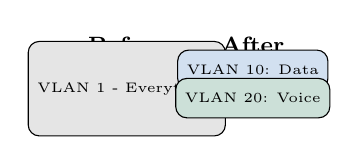
\begin{tikzpicture}[scale=0.4]
                    % Before
                    \node[font=\footnotesize] at (0, 2.8) {\textbf{Before}};
                    \node[draw, fill=gray!20, rounded corners, minimum width=1.8cm, 
                          minimum height=1.2cm, font=\tiny] at (0, 1.4) {VLAN 1 - Everything};
                    
                    % After
                    \node[font=\footnotesize] at (4, 2.8) {\textbf{After}};
                    \node[draw, fill=tcpblue!20, rounded corners, minimum width=1.6cm, 
                          minimum height=0.5cm, font=\tiny] at (4, 2) {VLAN 10: Data};
                    \node[draw, fill=paddysgreen!20, rounded corners, minimum width=1.6cm, 
                          minimum height=0.5cm, font=\tiny] at (4, 1.1) {VLAN 20: Voice};
                \end{tikzpicture}
            \end{center}
        \end{column}
        \begin{column}{0.48\textwidth}
            \begin{alertblock}{Key Lesson}
                \footnotesize
                Voice requires $<$150ms latency and minimal jitter. Without QoS, it competes equally with all other traffic!
            \end{alertblock}
        \end{column}
    \end{columns}
\end{frame}

% =============================================================================
% SLIDE 36: DR and HA Concepts Overview
% =============================================================================
\begin{frame}{Disaster Recovery and High Availability Concepts}
    \begin{columns}[T]
        \begin{column}{0.48\textwidth}
            \begin{block}{Key Definitions}
                \footnotesize
                \begin{itemize}\setlength{\itemsep}{1pt}
                    \item \textbf{DR}: Getting back to normal \textit{after} a failure
                    \item \textbf{HA}: Preventing downtime \textit{before} it happens
                    \item \textbf{BC}: Keeping operations running during disruption
                \end{itemize}
            \end{block}
            
            \begin{block}{The ``Nines'' of Availability}
                \footnotesize
                \begin{tabular}{@{}l c@{}}
                    \toprule
                    \textbf{Availability} & \textbf{Downtime/Year} \\
                    \midrule
                    99\% (two 9s) & 3.65 days \\
                    99.9\% (three 9s) & 8.76 hours \\
                    99.99\% (four 9s) & 52.6 min \\
                    99.999\% (five 9s) & 5.26 min \\
                    \bottomrule
                \end{tabular}
            \end{block}
        \end{column}
        \begin{column}{0.48\textwidth}
            \begin{center}
                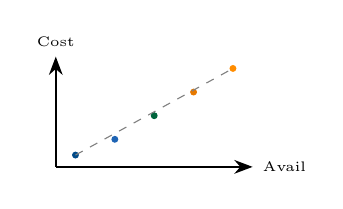
\begin{tikzpicture}[scale=0.5]
                    % Availability spectrum
                    \draw[-{Stealth}, thick] (0, 0) -- (5, 0) node[right, font=\tiny] {Avail};
                    \draw[-{Stealth}, thick] (0, 0) -- (0, 2.8) node[above, font=\tiny] {Cost};
                    
                    % Points
                    \fill[rctcblue] (0.5, 0.3) circle (2.5pt);
                    \fill[tcpblue] (1.5, 0.7) circle (2.5pt);
                    \fill[paddysgreen] (2.5, 1.3) circle (2.5pt);
                    \fill[aborange] (3.5, 1.9) circle (2.5pt);
                    \fill[sunnyorange] (4.5, 2.5) circle (2.5pt);
                    
                    % Trend line
                    \draw[dashed, gray] (0.5, 0.3) -- (4.5, 2.5);
                \end{tikzpicture}
            \end{center}
            
            \begin{alertblock}{Cost vs Availability}
                \footnotesize
                Each additional ``nine'' roughly \textbf{10x the cost}! Match availability to business needs.
            \end{alertblock}
        \end{column}
    \end{columns}
\end{frame}

% =============================================================================
% SLIDE 37: Disaster Recovery Metrics
% =============================================================================
\begin{frame}{Disaster Recovery Metrics}
    \begin{columns}[T]
        \begin{column}{0.48\textwidth}
            \begin{block}{Key DR Metrics}
                \small
                \begin{itemize}\setlength{\itemsep}{3pt}
                    \item \textbf{RTO} (Recovery Time Objective): Maximum acceptable \textit{downtime}
                    \item \textbf{RPO} (Recovery Point Objective): Maximum acceptable \textit{data loss}
                    \item \textbf{MTTR} (Mean Time To Repair): Average repair time
                    \item \textbf{MTBF} (Mean Time Between Failures): Reliability measure
                \end{itemize}
            \end{block}
        \end{column}
        \begin{column}{0.48\textwidth}
            \begin{center}
                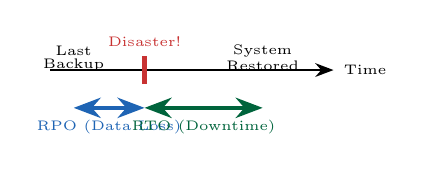
\begin{tikzpicture}[scale=0.6]
                    % Timeline
                    \draw[-{Stealth}, thick] (0, 0) -- (6, 0) node[right, font=\tiny] {Time};
                    
                    % Disaster marker
                    \draw[alertred, line width=2pt] (2, -0.3) -- (2, 0.3);
                    \node[font=\tiny, alertred] at (2, 0.6) {Disaster!};
                    
                    % RPO
                    \draw[{Stealth}-{Stealth}, tcpblue, line width=1.5pt] (0.5, -0.8) -- (2, -0.8);
                    \node[font=\tiny, tcpblue] at (1.25, -1.2) {RPO (Data Loss)};
                    
                    % RTO
                    \draw[{Stealth}-{Stealth}, paddysgreen, line width=1.5pt] (2, -0.8) -- (4.5, -0.8);
                    \node[font=\tiny, paddysgreen] at (3.25, -1.2) {RTO (Downtime)};
                    
                    % Last backup
                    \node[font=\tiny] at (0.5, 0.4) {Last};
                    \node[font=\tiny] at (0.5, 0.1) {Backup};
                    
                    % Recovery
                    \node[font=\tiny] at (4.5, 0.4) {System};
                    \node[font=\tiny] at (4.5, 0.1) {Restored};
                \end{tikzpicture}
            \end{center}
            
            \vspace{0.2em}
            \begin{block}{Example Metrics by System}
                \small
                \begin{tabular}{@{}l c c@{}}
                    \toprule
                    \textbf{System} & \textbf{RPO} & \textbf{RTO} \\
                    \midrule
                    Email & 24 hrs & 4 hrs \\
                    E-commerce & 1 hr & 15 min \\
                    Trading & Real-time & Seconds \\
                    \bottomrule
                \end{tabular}
            \end{block}
        \end{column}
    \end{columns}
\end{frame}

% =============================================================================
% SLIDE 38: Disaster Recovery Sites
% =============================================================================
\begin{frame}{Disaster Recovery Sites}
    \begin{block}{DR Site Types Comparison}
        \small
        \begin{tabular}{@{}l c c c c@{}}
            \toprule
            \textbf{Site Type} & \textbf{Equipment} & \textbf{Data} & \textbf{Recovery Time} & \textbf{Cost} \\
            \midrule
            \textbf{Cold Site} & None & None & Days--Weeks & \$ \\
            \textbf{Warm Site} & Partial & Recent backup & Hours--Days & \$\$ \\
            \textbf{Hot Site} & Full & Real-time sync & Minutes & \$\$\$ \\
            \textbf{Cloud DR} & On-demand & Replicated & Minutes--Hours & \$\$--\$\$\$ \\
            \bottomrule
        \end{tabular}
    \end{block}
    
    \begin{columns}[T]
        \begin{column}{0.32\textwidth}
            \begin{alertblock}{Cold Site}
                \small
                Empty facility with power/network. Must ship and install all equipment. Cheapest but slowest recovery.
            \end{alertblock}
        \end{column}
        \begin{column}{0.32\textwidth}
            \begin{block}{Warm Site}
                \small
                Some equipment pre-installed. Need to restore data from backups. Balance of cost and speed.
            \end{block}
        \end{column}
        \begin{column}{0.32\textwidth}
            \begin{exampleblock}{Hot Site}
                \small
                Fully operational mirror. Real-time data replication. Immediate failover. Most expensive.
            \end{exampleblock}
        \end{column}
    \end{columns}
\end{frame}

% =============================================================================
% SLIDE 39: Fault Tolerance, Redundancy, and Load Balancing
% =============================================================================
\begin{frame}{Fault Tolerance, Redundancy, and Load Balancing}
    \begin{columns}[T]
        \begin{column}{0.48\textwidth}
            \begin{block}{Redundancy Technologies}
                \small
                \begin{itemize}\setlength{\itemsep}{2pt}
                    \item \textbf{RAID}: Redundant disk arrays
                    \item \textbf{NIC Teaming}: Multiple network adapters
                    \item \textbf{Dual PSU}: Redundant power supplies
                    \item \textbf{UPS}: Uninterruptible power
                    \item \textbf{Multipathing}: Multiple storage paths
                \end{itemize}
            \end{block}
            
            \vspace{0.2em}
            \begin{block}{RAID Levels}
                \small
                \begin{tabular}{@{}l c l@{}}
                    \toprule
                    \textbf{RAID} & \textbf{Min} & \textbf{Tolerance} \\
                    \midrule
                    RAID 0 & 2 & None (striping) \\
                    RAID 1 & 2 & 1 disk (mirror) \\
                    RAID 5 & 3 & 1 disk (parity) \\
                    RAID 10 & 4 & 1 per mirror \\
                    \bottomrule
                \end{tabular}
            \end{block}
        \end{column}
        \begin{column}{0.48\textwidth}
            \begin{block}{Load Balancing Methods}
                \small
                \begin{itemize}\setlength{\itemsep}{1pt}
                    \item \textbf{Round Robin}: Rotate through servers
                    \item \textbf{Least Connections}: Send to least busy
                    \item \textbf{IP Hash}: Same client → same server
                    \item \textbf{Weighted}: Based on server capacity
                \end{itemize}
            \end{block}
            
            \vspace{0.2em}
            \begin{center}
                \begin{tikzpicture}[scale=0.5]
                    % Load balancer
                    \node[draw, fill=aborange!20, rounded corners, 
                          minimum width=1.5cm, minimum height=0.6cm, font=\tiny] (lb) at (0, 1.5) {Load Balancer};
                    
                    % Servers
                    \node[server] (s1) at (-1.5, 0) {\iconserver[0.3cm]};
                    \node[server] (s2) at (0, 0) {\iconserver[0.3cm]};
                    \node[server] (s3) at (1.5, 0) {\iconserver[0.3cm]};
                    
                    % Connections
                    \draw[-{Stealth}] (lb) -- (s1);
                    \draw[-{Stealth}] (lb) -- (s2);
                    \draw[-{Stealth}] (lb) -- (s3);
                    
                    % Health checks
                    \node[font=\tiny, paddysgreen] at (-1.5, -0.5) {\faCheck};
                    \node[font=\tiny, paddysgreen] at (0, -0.5) {\faCheck};
                    \node[font=\tiny, alertred] at (1.5, -0.5) {\faTimes};
                \end{tikzpicture}
            \end{center}
            
            \begin{alertblock}{Health Checks}
                \small
                Load balancers monitor server health and remove failed servers from the pool automatically!
            \end{alertblock}
        \end{column}
    \end{columns}
\end{frame}

% =============================================================================
% SLIDE 40: First Hop Redundancy Protocols (FHRP)
% =============================================================================
\begin{frame}{First Hop Redundancy Protocols (FHRP)}
    \begin{columns}[T]
        \begin{column}{0.48\textwidth}
            \begin{block}{The Problem}
                \footnotesize
                Clients use a single \textbf{default gateway}. If that router fails, clients lose connectivity!
            \end{block}
            
            \begin{block}{FHRP Comparison}
                \footnotesize
                \begin{tabular}{@{}l c c@{}}
                    \toprule
                    \textbf{Protocol} & \textbf{Vendor} & \textbf{Load Bal} \\
                    \midrule
                    HSRP & Cisco & No \\
                    VRRP & Open & No \\
                    GLBP & Cisco & Yes \\
                    \bottomrule
                \end{tabular}
            \end{block}
            
            \begin{exampleblock}{How It Works}
                \footnotesize
                Routers share a \textbf{Virtual IP (VIP)}. Clients point to VIP; active router responds. If active fails, standby takes over!
            \end{exampleblock}
        \end{column}
        \begin{column}{0.48\textwidth}
            \begin{center}
                \begin{tikzpicture}[scale=0.55]
                    % Routers
                    \node[router] (r1) at (0, 2) {\iconrouter[0.4cm]};
                    \node[font=\tiny] at (0, 1.4) {Active .2};
                    
                    \node[router] (r2) at (3, 2) {\iconrouter[0.4cm]};
                    \node[font=\tiny] at (3, 1.4) {Standby .3};
                    
                    % Virtual IP
                    \node[draw=paddysgreen, fill=paddysgreen!20, rounded corners, 
                          minimum width=1.8cm, font=\tiny] (vip) at (1.5, 3) {VIP: .1};
                    
                    % Client
                    \node[pc] (client) at (1.5, -0.3) {\iconpc[0.4cm]};
                    \node[font=\tiny] at (1.5, -0.9) {Gateway: .1};
                    
                    % Connections
                    \draw[dashed, paddysgreen] (vip) -- (r1);
                    \draw[dashed, gray] (vip) -- (r2);
                    \draw[-{Stealth}, paddysgreen, line width=1.5pt] (client) -- (1.5, 0.6) -- (r1);
                    
                    % Heartbeat
                    \draw[{Stealth}-{Stealth}, aborange, dashed] (r1) -- (r2) 
                        node[midway, above, font=\tiny] {Heartbeat};
                \end{tikzpicture}
            \end{center}
            
            \begin{alertblock}{Transparent Failover}
                \footnotesize
                Clients \textbf{never change} their gateway---FHRP handles failover automatically!
            \end{alertblock}
        \end{column}
    \end{columns}
\end{frame}

% =============================================================================
% SLIDE 41: Case Study - Frank's Foolproof Business Continuity Plan
% =============================================================================
\begin{frame}{Case Study: Frank's Foolproof Business Continuity Plan}
    \begin{casestudy}{``The Gang Needs Uptime''}
        \footnotesize
        Frank insists Paddy's Pub needs ``five nines'' availability for the new POS system after losing a full day of sales during the last power outage.
        
        \vspace{0.1em}
        \textbf{Current setup:} Single server, no automated backups (Charlie ``sometimes'' copies files), one budget ISP, no UPS.
        
        \vspace{0.1em}
        Frank's budget: ``As little as possible!''
    \end{casestudy}
    
    \begin{casesolution}{Realistic Improvements}
        \footnotesize
        \begin{enumerate}\setlength{\itemsep}{0pt}
            \item \textbf{UPS} (\$150--300): Immediate protection, graceful shutdown
            \item \textbf{Automated backups} (\$0--50/mo): Cloud backup for RPO
            \item \textbf{Secondary ISP} (\$50--100/mo): If budget allows
            \item \textbf{Realistic target}: 99.9\% (three nines)---five nines costs five figures!
        \end{enumerate}
    \end{casesolution}
\end{frame}

% =============================================================================
% SLIDE 42: Module 7 Summary and Port Reference
% =============================================================================
\begin{frame}{Module 7 Summary and Port Reference}
    \begin{columns}[T]
        \begin{column}{0.48\textwidth}
            \begin{block}{Key Protocols by Section}
                \footnotesize
                \textbf{7.1 Security/Time}: TLS (443), NTP (123), PTP (319/320)
                
                \vspace{0.2em}
                \textbf{7.2 Web/File}: HTTP (80), HTTPS (443), FTP (20/21), SFTP (22), SMB (445)
                
                \vspace{0.2em}
                \textbf{7.3 Email/Voice}: SMTP (25/587), IMAP (143/993), POP3 (110/995), SIP (5060)
                
                \vspace{0.2em}
                \textbf{7.4 DR/HA}: RTO, RPO, RAID, FHRP (HSRP/VRRP/GLBP)
            \end{block}
            
            \vspace{0.2em}
            \begin{alertblock}{Exam Reminders}
                \footnotesize
                \begin{itemize}\setlength{\itemsep}{0pt}
                    \item SFTP = SSH (port 22), not FTP!
                    \item Disable SMB1 (security)
                    \item Voice QoS: DSCP EF (46)
                    \item IMAP = server storage, POP3 = download
                \end{itemize}
            \end{alertblock}
        \end{column}
        \begin{column}{0.48\textwidth}
            \begin{block}{Essential Port Reference}
                \footnotesize
                \begin{tabular}{@{}l c c@{}}
                    \toprule
                    \textbf{Service} & \textbf{Port} & \textbf{Proto} \\
                    \midrule
                    HTTP & 80 & TCP \\
                    HTTPS & 443 & TCP \\
                    FTP & 20/21 & TCP \\
                    SSH/SFTP & 22 & TCP \\
                    SMTP & 25, 587 & TCP \\
                    POP3/S & 110, 995 & TCP \\
                    IMAP/S & 143, 993 & TCP \\
                    NTP & 123 & UDP \\
                    SMB & 445 & TCP \\
                    MySQL & 3306 & TCP \\
                    SIP & 5060/5061 & Both \\
                    \bottomrule
                \end{tabular}
            \end{block}
        \end{column}
    \end{columns}
\end{frame}

\end{document}